\documentclass[12pt,final]{report} % for letter size paper
% 215.9mm × 279.4mm

\usepackage{ifxetex}
\usepackage[T1]{fontenc}
\usepackage[utf8]{inputenc}

\usepackage[french]{babel}
\usepackage{tikz, titling, background, setspace}
\usepackage[left=.5in,right=0.5in,top=0.6in,bottom=.525in,a5paper]{geometry}

\usepackage{mathrsfs}
\usepackage{textpos}
\usepackage{comment}

\usetikzlibrary{calc}
\usetikzlibrary{shapes}
\usetikzlibrary{backgrounds}
%\tikzstyle{block} = [rectangle, draw, fill=blue!20, text width=5em, text centered, rounded corners, minimum height=4em] 
\tikzstyle{line} = [draw, text centered]
%\tikzstyle{output} = [fill=white]

\definecolor{textcolorPencil}{rgb}{0.99,0.69,0.07}


\newcommand{\stardelimiter}{
\[ \star \star \star \]
\newpage
%\begin{minipage}[][\baselineskip]{\textwidth}
	%\hrule
%\end{minipage}
}

\newcommand{\datemarge}[1]{%
   \newpage
    %\begin{textblock}{3}(-3.1,0)
        {\color{blue}#1}
    %\end{textblock}

}

%\renewcommand{\rmdefault}{augie}
%\fontfamily{French Cursive}
\usepackage{frcursive}
\DeclareTextFontCommand{\helvetica}{\fontfamily{phv}\selectfont}
\renewcommand{\rmdefault}{frc}

\newcommand{\majuscule}[1]{\emph{\texttt{#1}}}
\newcommand{\sentence}[1]{\item «#1»}
\newenvironment{dialogue}{\begin{itemize}}{\end{itemize}}


\title{Quand la logique s'en mêle}
\author{Alexandre Janniaux}

\begin{document}
  %\pagestyle{empty}
\doublespacing{}
  %\kant[1-6]{}

  \maketitle

  \backgroundsetup{%
 angle=0,
 scale=1,
 placement=bottom,
 contents={%
     \begin{tikzpicture}[overlay]%
         [
             normal line/.style={gray, very thin},
             every node/.append style={black, align=center, opacity=1}
         ]
         \begin{scope}[on background layer]
             %\foreach \y in {1,2,...,10} {
             %  \draw[line] (0,0.71\y) -- (8.5in,0.71\y);
             %}
             %\node (t) [font=\LARGE, anchor=south] at ($(0,25.56)!1/2!(8.5in,25.56)$) {\thetitle};
             %\node (d) [font=\large, anchor=south west, xshift=1.5em] at (0,25.6) {\today};
             %\node (p) [font=\large, anchor=south east, xshift=-1.5em] at (8.5in,25.56) {p.~\thepage};
%             \draw[line,color=red] (1.16in,0) -- (1.16in,23in);
             \draw[line width=0.3pt,color=gray,step=0.5cm] (current page.south west) grid (current page.north east); % (0,-13in) grid (10in,10in);
             %\draw[line width=0.5pt] (0,1.4in) (10in,1.4in);
             %\foreach \y in {0.71,1.41,...,25.56}
             %  \draw[normal lines] (0,\y) -- (8.5in,\y);
             %\draw[normal lines] (1.25in,0) -- (1.25in,11in);
             %\node (t) [font=\LARGE, anchor=south] at ($(0,25.56)!1/2!(8.5in,25.56)$) {\thetitle};
             %\node (d) [font=\large, anchor=south west, xshift=1.5em] at (0,25.6) {\today};
             %\node (p) [font=\large, anchor=south east, xshift=-1.5em] at (8.5in,25.56) {p.~\thepage};
         \end{scope}
     \end{tikzpicture}%
     \begin{tikzpicture}[overlay]
         [
             normal line/.style={gray, very thin},
             every node/.append style={black, align=center, opacity=1}
         ]
         \begin{scope}[on background layer]
         \draw[line,color=red] (-2.95in,0) -- (-2.95in,23in);
     \end{scope}
     \end{tikzpicture}
}}



  
  {\setstretch{1.963} %\color{textcolorPencil}
  %\setstretch{2.1}
      \vspace{0pt}%\cursive{}

      %TODO: petite introduction du but de ce cahier, mettre une photo du cahier réel à la fin.

\datemarge{Le 12 octobre 2014}
Longue attente devant la porte de la salle de cours. 
Je discute non sans anxiété avec d'autres élèves de ma classe préparatoire --- taupins dans notre jargon --- qui vont bientôt subir le même sort que moi.
Quelle sensation étrange d'être anxieux pour la présentation d'un sujet que l'on connait probablement mieux que les autres?

Ça y est, la porte s'ouvre, je rentre. Un petit regard vers l'autre table, où l'on parle beaucoup trop physique pour mon esprit d'informaticien, et je m'asseois en face de mon professeur de mathématiques.

\begin{dialogue}
    \sentence{Bonjour Alexandre, comment allez vous?}
\end{dialogue}
% TODO: image M.Pauly

Si l'on vous dit un jour, comme pour moi, que les professeurs du Lycée du Parc sont arrogants, méprisants, et ne font qu'essayer de vous écraser, vous rierez de voir cette descritpion tomber devant ce professeur.


% FIXME: Typo Dialogue
\begin{dialogue}
    \sentence{Venons-en à ce pourquoi vous êtes ici, racontez-moi ce que vous faîtes.}

    \sentence{Oui! J'ai choisi un sujet d'informatique sur l'optimisation de la planification aérienne. On part d'un certain nombre d'avions, d'aéroports et de clients, et il faut trouver les meilleures configurations des vols en fonction de plusieurs critères.}

    \sentence{C'est ambitieux comme sujet, vous savez comment vous y prendre?} % FIXME : lyon "y"

    \sentence{En réalité, j'ai surtout choisi ce sujet comme prétexte à l'utilisation d'algorithmes génétiques.}

    \sentence{Et vous avez déjà codé ce genre d'algorithme?.}

    \sentence{Oui, évidemment.}
\end{dialogue}

Pas besoin de dire que c'est le stress qui a répondu à ma place, même si j'aurai été capable d'expliquer le fonctionnement de l'algorithme.

\begin{dialogue}
    \sentence{Dans l'état actuel, une seule chose m'inquiète. 
    J'ai l'impression que je ne fais rien de théorique, et qu'expliquer le fonction de ces algorithmes sera non seulement pauvre, mais me prendra aussi tout mon temps de parole.}

    \sentence{Qu'est-ce que vous aimeriez ajouter?}

    \sentence{J'avais l'idée de mieux formaliser l'algorithme dans ce cas là et de montrer que l'on converge probablement vers un optimum.}

    \sentence{Vous savez, il vous reste beaucoup de temps, et vous n'avez pas encore énormément de recul sur votre projet.
        Attendez un peu: à force de vivre avec le problème, vous serez à même de l'expliquer clairement et rapidement.
        Essayez de simplifier ce problème d'abord.}

    \sentence{D'accord, ça me parait rapide à faire.}
\end{dialogue}

\stardelimiter{}

Les algorithmes génétiques sont des programmes extraordinaires qui font partie de la classe des méta-heuristiques, alias algorithmes tout terrain pour les intimes. 
Ils sont capables de résoudre un problème sans vraiment en connaître les caractéristiques et fonctionnent grâce aux dures loi de l'évolution mises en lumière par Darwin, en particulier la sélection naturelle. 
L'algorithme semble aussi fou qu'il est efficace.
Son fonctionnement peut être très simple à décrire: 
Imaginons que l'on tape plusieurs textes totalement aléatoires, en jetant des billes sur un clavier par exemple.
Prenons alors tous ces textes pour les faire lire à une communauté de lecteurs passionnés, qui va objectivement leur donner une note.
Reprenons ensuite les textes un par un, lançons une pièce, et s'il s'agit d'un pile, modifions aléatoirement une lettre dans le texte.
Sélectionnons alors les meilleurs textes, découpons une partie dans chacun d'entre eux, que l'on échange avec un autre texte considéré meilleur que les autres.
Puis on recommence le processus: c'est un vrai bazar. 
Et pourtant, c'est exactement ce que font les algorithmes génétiques.
Et évidemment, c'est diaboliquement efficace, sous réserve que la communauté de lecteurs sache correctement noter les textes, et dispose d'un mental d'acier pour lire tous ces pseudo-textes.
%TODO: exemple robot qui se combattent ? si il y a de la place

\stardelimiter{}

\datemarge{Le 1er novembre 2014}

%TODO: Separator line
Il est déjà 19 heures, j'ai réuni toutes les sources dont j'ai besoin pour mon projet. 
C'est étrange de ressortir ce Linux Pratique Essentiel, le magazine qui m'a poussé vers cette idée de sujet. 
En soi, c'est assez difficile de choisir un sujet sur lequel travailler pendant plus d'un an, avant même de le connaître,
et j'étais assez content d'être tombé dessus.
Lorsque j'avais choisi mon sujet, en fin de première année de prépa, j'avais été aidé par un ami, maintenant en thèse d'apprentissage et robotique.
Après un long brainstorming sur comment développer le sujet imposé cette année, j'avais fait ressortir deux projets assez imposants.
Le premier, c'était bien sûr celui sur la planification aérienne. 
Quant au second, il s'agissait encore d'un problème d'optimisation, mais qui demandait de développer une intelligence à base de réseaux de neurones pour optimiser la consommation énergétique des datacenters, à l'instar de ce que fait Google.

J'ai acheté des livres également, \textit{A Field Guide to Genetic Programming} qui risque de m'accompagner longtemps.
Mais je m'étais également intéressé au livre de Cédric Villani, \textit{Théorème Vivant}, pour renouer avec mon envie de faire des maths et enfin lire son travail de vulgarisation. 
Mmmmh, l'heure tourne, je devrai peut être dormir, cette semaine encore va être longue à vivre\dots

\datemarge{Le 24 novembre 2014}

%TODO Separator line
Toujours aucune issue en vue!
Je cherche désespérément comment améliorer mon sujet et le rendre intéressant, je n'arriverai pas à le présenter autrement!
Pourtant je ne l'ai même pas encore commencé, l'enthousiasme que j'avais en choisissant ce projet s'est très vite envolé avec le début de cette année.
Enfin bon, pas le temps de culpabiliser, là tout de suite, c'est pause détente. 

La cafétéria du lycée est toujours autant peuplée, mais le flux s'estompe progressivement lorsque les lycéens ont trouvé de quoi manger et qu'ils retournent travailler. 
De mon côté, je continue de lire \textit{A Field Guide to Genetic Programming}, cette passion-là ne s'est pas arrêtée au moins.
% FIXME : le -- est pas génial pour écrire
Un de mes co-trinômes --- ce groupe composé de trois amis soudés pour affronter les examens au tableau deux fois par semaine --- commence à s'intéresser un peu à ce que je fais.

\begin{dialogue}
    \sentence{C'est pour ton \majuscule{TIPE}, non?}

    \sentence{Oui\dots en quelque sorte! il faut que j'utilise ces algorithmes pour un problème d'optimisation.}

    \sentence{J'en ai déjà entendu parler, mais je n'ai jamais compris comment ça fonctionnait, finalement.}

    \sentence{C'est assez simple, tu pars d'une population de solution initiale arbitraire, et tu la fais évoluer en fusionnant les caractéristiques chez les bons individus et en gardant les meilleurs, en gros.}

    \sentence{Ah oui\dots et tu peux t'en servir pour n'importe quoi, du moment que tu peux représenter les individus?}

    \sentence{Pas seulement, il faut aussi avoir une bonne fonction pour leur attribuer des notes, qui soit suffisamment expressive sans demander trop de temps. Mais ça a été utilisé pour faire des antennes pour la {NASA}. Attends je dois avoir une photo quelque part\dots là, voilà!}

    \sentence{C'est assez atypique comme antenne, en effet!}

    \sentence{Là aussi, il y a un autre exemple avec la génération de circuits électriques pour obtenir une certaine fonctionnalité, et ça doit être possible de forcer l'algorithme pour qu'il réalise des circuits de taille minimale.}
\end{dialogue}

Me voilà reparti dans ma lecture.

\vspace{-0.1cm}

\stardelimiter{}

%TODO: texte avec l'image de l'antenne et une explication du travail de Holand et des algorithmes génétiques.
\vspace{0.1cm}

\begin{figure}[h]
    \centering
    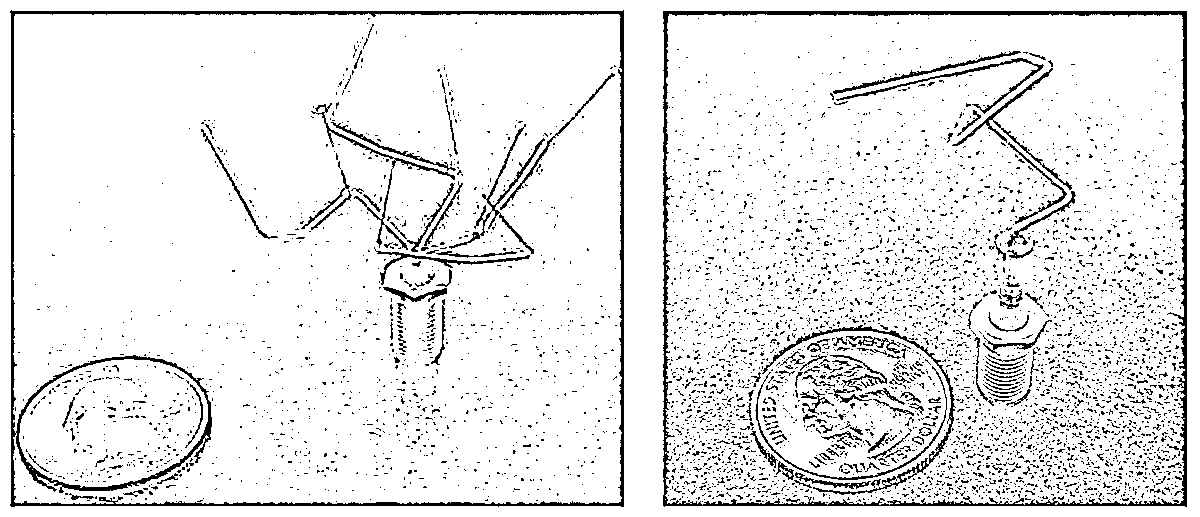
\includegraphics[width=13cm]{GeneticallyGrownAntennas_NASA-web.png} %TODO source 
    \caption{Antennes obtenues par évolution génétique}
\end{figure}

\vspace{-1cm}

\stardelimiter{}

%\vspace{0.36cm}

\newpage

\datemarge{Le 9 décembre 2014}%FIXME

Ah les mardis, quelle épreuve! 
Encore une fois, impossible de rester concentré sur le cours en informatique, malgré mon intérêt pour le sujet!
Conséquence malheureuse d'un jour devenu le jour devenu moment de gastronomie entre amis. % FIXME
Bon, après tout, ca reste assez agréable d'avoir cette pause de deux heures le midi: la sensation typique de ne pas avoir de temps des classes préparatoires s'évanouit dans un bon moment de détente et permet d'assurer une forme correcte tous les jours.
Mais je suis totalement incapable de suivre ce cours de logique sans me laisser distraire!

Je regarde le cours qu'on nous a donné: forme normale conjonctive, lois de De Morgan, table de vérité, évaluation\dots
Mouais, c'est quand même pas très sexy comme sujet de toute façon, et ça n'a pas l'air très dur à travailler.
Pendant que je surligne les passages importants sur le cours livré en diapositives imprimées, j'essaye d'imaginer de quelle façon présenter mon projet:
il me faut non seulement des idées pour rendre la présentation vivante, avec des expériences et applications concrètes et sympathiques, mais également que je puisse montrer ma connaissance du sujet.
C'est un grand défi de montrer tout ça en seulement dix minutes, ou quarante si je réussis à passer les \majuscule{ENS}.
Éventuellement, je n'ai qu'à présenter les résultats en mentionnant que je l'ai résolu avec un algorithme génétique, et présenter d'autres résultats théoriques sur le problème ou encore la convergence du programme?
Ça me donne l'impression de bidouiller ma présentation pour que ça colle à ce qu'on me demande, ça ne me plaît pas trop.
Ou alors, je mentionne plusieurs fois que j'ai travaillé sur le côté théorique et je profite du temps alloué pour les questions pour développer selon ce qui intéresse le jury?
Mmmh, pari risqué encore une fois.

C'est fou que je n'ai toujours pas la moindre idée de comment présenter ça après tout ce temps, même si j'en ai encore beaucoup.

Hop reprise du cours, je parle encore avec mon co-trinôme.
\begin{dialogue}
    \sentence{Ce sont presque que des choses qu'on fait en sciences de l'ingénieur en terminale}.
    \sentence{Oui, je crois même qu'on fait ça en classe de sup aussi.}
    \sentence{En plus, c'est plutôt intuitif. De Morgan, par exemple, c'est juste une histoire de Français.}
    \sentence{Ah, je la connais par c\oe{}ur moi, c'est tout. Je sais juste que c'est ça.}
\end{dialogue}

Il écrit la formule sur le cours pour me la montrer, je suis assez étonné de sa réponse.
%FIXME 
%TODO : afficher la formule
\begin{dialogue}
    \sentence{Mais tu ne l'interprètes pas du tout comme du Français?}
    \sentence{Non? Pourquoi, comment est-ce que tu l'interprètes toi?}
    \sentence{garde, le membre de gauche, c'est que tu n'as aucun de A ou B, et le membre de droite, que tu n'as ni A, ni B. C'est un peu de la distributivité de la négation si tu l'exprimes en Français.}
    \sentence{Ah\dots Oui\dots C'est assez cool en fait! Et tu as déjà vu les tableaux de Karnaugh?}
    \sentence{Carnot? Pour la thermodynamique?}
    \sentence{Non, non, pas ce Carnot-là. Celui pour simplifier les expressions logique.}
    \sentence{Ça me dit quelque chose, peut-être que j'en ai entendu parler en \majuscule{SI} l'année dernière.}
    \sentence{Regarde. Je te le montre avec quatre variables. Avec plus c'est plus vraiment pratique. Tu fais un tableau à deux entrées. Tu mets tes variables ici et là, tu mets le résultat du calcul ici, et tu fais des paquets avec tous les 1 pour avoir la forme simplifiée.}
    \sentence{Euh\dots oui, mais comment tu remplis ce tableau?}
    \sentence{Il suffit de faire le calcul entre les différentes variables.}%TODO
    \sentence{Mmmh, oui, d'accord, et pour les 1, pourquoi tu ne fais pas des lignes de trois 1 ici, ça fait moins de blocs!}
    \sentence{Il faut que ton rectangle ait des côtés de longueur une puissance de deux pour que ça marche, mais par contre ton tableau est comme une sphere, tu peux faire un carré avec les 4 coins ou le commencer sur un bord et prendre l'autre bord avec.}
    \sentence{Mmmh, d'accord.}
\end{dialogue}

J'espère qu'il ne le saura pas, mais je n'ai pas compris grand chose à son tableau. 
Ça ressemble plus à de l'informagie vaudou qu'à une vraie technique de minimisation pour moi, et il y a beaucoup de contraintes étranges sur la réalisation du tableau.
Néanmoins, je garde cette technique en tête, il faudra que je revienne dessus lorsque j'aurais un peu plus de temps.

\datemarge{Le 26 décembre}

\begin{comment}
%TODO: réécrire cette partie
Aujourd'hui, je ne sais vraiment plus quoi faire pour ce projet, rien ne correspond à ce que je veux.
J'ai fini par penser que je n'arriverai pas à terminer à temps.
Il est temps de prendre des mesures pour améliorer cela.
%TODO expliquer pourquoi
Peut être faire un projet en physique, c'est censé être plus facile? Si seulement je pouvais en comprendre quelque chose!
Ou alors un sujet de mathématiques? 
Il faut seulement que je me débarrasse de cette impression de ne rien faire moi-même. 

Je suis encore sur Internet, l'autoplay de youtube a fini par m'amener de vidéos d'algorithmes génétiques appliqués au jeu vidéo, à des vidéos de pendule doubles --- à deux tiges --- asservi par un moteur. 
\end{comment}

%FIXME: date, séparer en deux ou pas ?
Enfin les vacances de Noël, je ne prendrai pas plus de travail en retard que ce que j'ai déjà. 
En revanche, pas le temps de souffler, j'ai beaucoup à faire, et je veux commencer à programmer le c\oe{}ur du solveur pour le projet.
Mais je ne m'empêche pas de regarder quelques vidéos intéressantes, surtout que c'est à propos de mon sujet favori.
Je regarde une vidéo de démonstration mélangeant réseaux de neurones et algorithmes génétiques afin d'entrainer deux créatures au comportement simplifié à se battre.
%TODO: image + développer

La vidéo suivante m'interpelle également.
Il s'agit encore du même type de système, mais pour entrainer une créature à sauter le plus loin possible, avec des membres définis par l'utilisateur avant la simulation.
C'est assez incroyable de voir à quel point cela fonctionne bien.
Les créatures ne savent rien de leur environnement, et ne savent pas comment elles fonctionnent au début de la simulation, mais finissent par avoir un comportement «rationnel» de manière naturelle.
%TODO: image + développer

%TODO: vidéo screensaver avec les créatures qui doivent apprendre à bouger + araignée qui apprend à rester stable.

Beaucoup de vidéos finissent par passer, et je me retrouve alors par hasard devant une vidéo d'un cube assez spécial qui éveille mon imagination. 
Il s'agit d'un cube programmable assez petit, dont l'intérieur contient des masses qu'il fait tourner, puis qu'il bloque afin de bouger.%FIXME redaction
En soit, le principe de ce cube est vraiment simple, mais j'y vois alors un océan de nouvelles possibilités.

Imaginons seulement que ces cubes sont munis d'électroaimants sur leurs faces, ainsi que de crochets actionnables. 
Nous pourrions alors manipuler les cubes comme des composants qui s'assemblent entre eux.
Plus encore, si nous munissons ces cubes de moyen de communication à courte distance, et que nous créons différents «modules de cube» comme une rotule, une batterie supplémentaire, un panneau solaire, des crochets, une caméra, des systèmes de traitement et tout ce qui peut être utile à une situation donnée, nous pourrions utiliser tous ces modules pour créer un système fonctionnant comme un robot modulaire, qui peut s'adapter à toute situation pour progresser dans un terrain inconnu.
Ce serait la solution à des problèmes comme envoyer un robot dans les centrales nucléaires de Fukushima afin de contrôler les problèmes, plutôt que d'envoyer des robots qui souvent ne peuvent effectuer la tâche demandée.

Cette idée me plaît beaucoup; même si elle n'est en pratique pas très réalisable, elle apporte un socle consistant aux travaux que je peux faire dessus.%TODO qualités du sujet
Mmmh, et si je changeais de sujet de \majuscule{TIPE}? Ai-je vraiment le temps de recommencer à partir de zéro?
Quelle partie du sujet traiter? 

Je m'empresse de sortir une feuille. Il n'y a rien de mieux qu'un brouillon papier pour développer une idée. 
Ça me rappelle la carte heuristique que j'avais fait en première année pour m'approprier le thème et développer quelques idées de sujet.

Il y a beaucoup de techniques pour penser à de nouvelles idées.%fixme
Celle de la carte heuristique (aussi appelée carte des idées, ou mind map) a le grand avantage d'être très visuelle, et met en valeur l'idée bien plus que sa précision. 
Que faut-il mettre dans une carte heuristique, et même de quelle manière cet outil permet d'avancer dans une recherche d'idée?
De mon expérience, cela n'apportera jamais de nouvelles idées, donc l'intérêt n'est pas de créer de nouveaux paramètres à prendre en compte.
Cela se comprend très bien en remarquant qu'il s'agit toujours de mots clés ou de dessins qui sont toujours reliés à des idées que l'on connait.
C'est la simplicité à relier ces ébauches d'idées entre eux qui fait la puissance de cet outil. 
Sa capacité d'organisation et d'archivage des idées en fait le compagnon idéal pour représenter une première approche de nos connaissances.
%TODO compléter, simplifier, rajouter image
%simplifier le problème en changeant de dimension %TODO plus tard pour le projet

Ça y est, j'ai une idée qui peut potentiellement utiliser les algorithmes génétiques. 
Pourquoi ne pas simuler un réseau de ces cubes, en simplifiant le déplacement et en me concentrant sur la création de leur comportement.
Je n'ai alors qu'à choisir une situation quelconque, avec une complexité intrinsèque suffisamment profonde pour ne pas être abordée de façon précise en classe préparatoire, par exemple la récupération de ressources en terrain inconnu.
Je vois déjà tout le système en image, avec des transporteurs, des caméras, des obstacles, des alimentations, \dots
Il va falloir que je prévienne mes professeurs, et que je trouve le vocabulaire qui correspond à ce sujet pour mes recherches.
%TODO: placer le mail + remplir ? 

\datemarge{Le 6 janvier 2015}

J'ai envoyé le mail, j'ai été plutôt flou sur la description de mon idée, et je vais aller voir mon professeur d'informatique pour développement.
Mon idée me fait vraiment penser à un jeu de stratégie, et ça me plaît beaucoup, mais je ne sais pas si mes professeurs et mon jury seront aussi réceptifs à ce projet.
\begin{dialogue}
	\sentence{Bonjour, vous m'aviez demandé de venir pour parler de mon \majuscule{TIPE}.}
	\sentence{Ah, oui bien sûr. Alors, pour changer de sujet, il n'y a évidemment pas de soucis, il faut juste le faire assez vite, avant de ne plus pouvoir remplir la fiche synoptique. Par contre, je n'ai pas très bien compris ce que tu veux faire exactement.}
\end{dialogue}

Et la machine se met en route.
On parle, on fait des gestes de main pour essayer de visualiser de la même chose, on gribouille sur le tableau, et on en arrive finalement à sa conclusion.
\begin{dialogue}
	\sentence{Mmmh, oui je vois maintenant, c'est intéressant. Mais il faut que  tu définisses mieux ton cadre. Quelles sont les contraintes, pourquoi tu veux utiliser un algorithme génétique, et même simplement de quelle manière tu comptes encoder le problème pour appliquer cet outil?}
	\sentence{Oui, ça je ne sais pas encore vraiment comment le faire.}
	\sentence{N'hésite pas à revenir me voir lorsque tu auras avancé là dessus.}
\end{dialogue}
D'un coup, encore une fois, je suis devenu beaucoup moins sûr de mon sujet.
Certes, il est intéressant, utilise les algorithmes génétiques, et plutôt drôle à expliquer à des gens, mais je me sens un peu étranger au problème maintenant que nous avons déterré beaucoup des questions importantes. 
Bon, je penserai à cela en détails plus tard, j'ai suffisamment de motivation pour aller courir, et il ne fait pas trop froid encore!

Rien de tel d'ailleurs que le bien connu Parc de la Tête d'Or à Lyon pour changer de l'enfermement de la prépa.
%TODO remplir
Je fais quand même un bilan de mon \majuscule{TIPE} pendant que je cours:
Finalement, je n'ai fait que choisir des projets assez complexe à formaliser, dans le but d'utiliser les algorithmes génétiques, pour finir démotiver en commençant à rentrer dans le sujet.
Peut être qu'un projet plus simple me permettra d'accrocher un peu plus et de mieux pouvoir le présenter?
Je vais aller voir si les deux pandas roux du Parc sont présents.
Traditionnellement ici, beaucoup de gens disent qu'avoir l'occasion de voir ces deux pandas sortir sur l'arbre apporte de la chance.
Et je crois bien qu'il m'en faut beaucoup!

\datemarge{Le 8 janvier 2015} %FIXME

Euréka! Pourquoi n'ai-je pas développé cette idée plus tôt!
En relisant «A Field Guide To Genetic Programming», je suis retombé sur la page à propos de la génération de circuits électriques\dots et c'est presque exactement ce qu'il me faut.
Je dois vite retourner voir mes professeurs pour qu'ils me valident un sujet sur ce thème!
Je dois juste réduire la partie «physique» qui ne m'intéresse pas beaucoup.
Pourquoi ne pas m'intéresser seulement aux circuits logiques, par exemple à comment les minimiser?
J'ai déjà de bonnes idées pour appliquer l'algorithme: par exemple en encodant les circuits comme un arbre, on peut facilement appliquer l'opérateur de crossover en copiant les fils n\oe{}uds à la même hauteur, ou en inversant un fils père et son fils n\oe{}ud.
Je peux aussi facilement faire une présentation intéressante en comparant des algorithmes naïfs et approximés qui donnent des solutions plus ou moins correcte en prenant plus ou moins de temps à l'algorithme génétique.
Si je suis capable de montrer que ce dernier peut trouver des solutions différentes et potentiellement plus intéressantes que les versions approximatives, et donner plus de souplesse sur les contraintes et le résultat voulu, je pense que j'aurai largement gagné pour la présentation.

Le problème est sûrement \majuscule{NP}-difficile de toute manière, donc l'algorithme génétique a bien sa place dans l'histoire, même si je ne peux pas allez aussi loin.

\stardelimiter{}

En informatique, on s'intéresse à la nature abstraite des problèmes, le nombre d'opérations à faire pour le résoudre, la place qu'ils requièrent en mémoire, son comportement en moyenne, dans le pire des cas, et bien plus encore.
On cherche en fait à les catégoriser, comme les mathématiques le feraient, et même étrangement les transformer l'un en l'autre. 
Ainsi, la résolution d'une partie de Tétris se ramène à la recherche d'un chemin Hamiltonien dans un graphe construit à partir de la partie, c'est-à-dire d'un chemin dans un graphe qui passe par tous les sommets de ce graphe une et une seule fois.
La théorie des langages donnent un cadre général d'étude pour les caractériser.
En particulier, parmi ces problèmes, deux classes sont particulièrement connu et ont beaucoup été étudiées.
On les appelle par les douces lettres \majuscule{P} et \majuscule{NP}, pour «Polynomiale» et «Non-déterministe Polynomial», et elles font même l'objet d'une question centrale mise à prix pour un million de dollars par le Clay Mathematics Institute grâce à un mécène souhaitant promouvoir et disséminer la connaissance dans le monde. 

La classe \majuscule{P} contient les problèmes qui ne deviennent pas trop difficile à résoudre lorsque le problème grossit, tandis que la classe \majuscule{NP} contient tous les problèmes pour lesquels il n'est pas trop difficile de vérifier qu'une solution donnée fonctionne bien.
Il est assez évident, lorsqu'on est assez familier, de voir que \majuscule{P} fait déjà partie de \majuscule{NP}, et même que l'on pourrait construire une hiérarchie, répondant au nom de «hiérarchie polynomiale», en considérant des presque-machines qui font comme si un problème normalement dans \majuscule{NP} était dans \majuscule{P} pour eux. 
La question mise à prix est maintenant de savoir si \majuscule{P=NP} ou non, et les chercheurs sont plutôt d'avis que non\dots


\datemarge{Le 18 février 2015} %TODO date

J'ai bien avancé dans mes recherches.
Bien évidemment je suis sur une ancienne connaissance, les fameux tableaux de Karnaugh dont m'avait tant parlé Antonin. 
Mais je m'intéresse plus spécialement à une autre technique, qui s'exécute de manière itérative et incrémentielle, et me semble moins magique que ces étranges tableaux.
Mais je ne comprend pas les explications associées à l'algorithme.
En fait, il est possible de caractériser tous les circuits par une fonction booléenne, c'est-à-dire une fonction qui ne connaît que les notions de vrai ou faux.
On peut même restreindre la fonction le circuit à une certaine forme sans perdre un chouïa de généralité pour ce problème.

Ce que je n'arrive pas à saisir, c'est la façon dont l'auteur a choisi de représenter graphiquement cet algorithme.
Pourquoi l'auteur fait-il une analogie avec un cube?
Il semble expliquer que ce cube représente une fonction, et donc un circuit, mais en quoi est-ce lié à l'algorithme?
Pourquoi ces opérations itératives ont un sens sur ce cube?

Je vais laisser ça de côté, allons revoir Antonin pour qu'il m'explique à nouveau les tableaux de Karnaugh.
Je sors de chez moi, et traverse la rue. 
Quoi de plus agréable que d'habiter en face de sa prépa, à côté du Parc de la Tête d'Or, et éviter les galères matinales avec les transports?
Alors que je rejoignais simplement les autres dans le préfabriqué qui nous sert de salle de travail, une idée fuse dans ma tête:
Le cube de tout à l'heure, généralisé à une dimension plus grande, possède un nombre de sommet qui est une puissance de deux!
Est-ce que c'est une coïncidence avec les limitations imposées sur les dimensions des carrées utilisés pour recouvrir les 1 dans le tableau de Karnaugh?
Mmmh, gardons cette idée au frais dans un coin, on verra si cela ressurgit pendant qu'Antonin m'explique une fois de plus sa méthode mystérieuse.

La suite, c'est quelque chose qui me plaît beaucoup dans la vie scientifique: 
Nous prenons des craies et attaquons impitoyablement le tableau pour démêler les pensées qui nous traversent et éradiquer toute trace de doute ou de questionnement.
Si la télépathie pouvait devenir possible, les sciences perdraient leur charme et leur attrait.

Après plusieurs dizaines de minutes à échanger nos idées et chercher la moindre faille dans nos pensées, je finis par lui parler de mon algorithme:

\begin{dialogue}
	\sentence{Bon, ce que je dois faire, c'est exactement la même chose que toi, mais l'algorithme fonctionne différemment.
	Je passe en forme normale conjonctive, que j'écris sous forme de 0 et de 1, je trie les termes selon leur nombre de 1 par ordre croissant et par groupe, et à chaque étape, je prend le plus petit groupe et je le fais fusionner avec celui d'après si c'est possible. 
	Chaque terme est un impliquant, et les termes qu'on obtient lorsqu'on ne peut plus simplifier sont appelés impliquants premiers.}
	\sentence{Euuh\dots peut être?}
	\sentence{Ça doit être difficile à voir! En fait, je cherche un lien entre Karnaugh et Quine-McCluskey. J'ai trouvé la forme de Blake sur internet, qui s'appelle aussi minimum covering set, mais je ne comprend pas vraiment ce que c'est. }% TODO
	\sentence{Après, ce que tu fais, ça ressemble beaucoup à Karnaugh. Dans Karnaugh on place les variables en binaire réfléchi pour que les 1 soient bien à côté, et tu vois cette étape? Ça doit correspondre à prendre ce rectangle dans Karnaugh.}
\end{dialogue}

Quel éclair de génie, c'est la clé. Le tableau de Karnaugh, c'est le cube que l'on a aplati.
Les 1 dans le tableau qui sont à côté sont également des termes qui sont adjacents dans le cube.
Je vais pouvoir commencer à préparer la présentation de mon projet!
Les choses s'accélèrent, nous allons bientôt commencer à faire les présentations devant un jury de professeur.

\datemarge{Le 27 avril 2015}

Soleil aveuglant, chaleur étouffante, j'ai vraiment bien fait de ne pas passer les écrits de Centrale Paris.
Mais l'environnement des concours me pousse à nerfs, j'ai peur de ne pas tout finir à temps!
Au moins, je commence à travailler des parties plus théoriques sur la complexité du problème, allant des façons naïves de l'aborder à des techniques bien moins naïves.
Je sens que ma pensée se précise au fil des éléments que je produis, mais il me manque du concret.

En allant à la bibliothèque universitaire de Lyon, j'ai pu trouver l'un des livres les plus magnifiques pour aborder l'étude des algorithmes. 
D'ailleurs, il est si renommé que beaucoup de gens l'appellent «Le Cormen» du nom d'un de ses auteurs, plutôt que par son nom «Introduction à l'algorithmique».
Une fois le livre posé sur la table excentrée de la \majuscule{BU}, je me décide à calculer le nombre de circuits que pourrait traiter l'algorithme naïf dans le pire des cas.
Après quelques dizaines de minutes de travail, je choisi enfin une approche récursive qui m'a l'air valide, en construisant des circuits plus grands à partir de ceux déjà générés et que l'on peut facilement énumérer.
%TODO schéma combinaison

Le résultat me parait difficile à interpréter, mais ça me semble déjà gigantesque. Est-ce une complexité exponentielle?
Bon simplifions, ça devrait être un peu moins que si je comptais les fonctions booléennes entre ces deux espaces, ce qui me donne rapidement\dots Quoi! deux puissance deux puissance n possibilités! Complexité en exponentielle d'exponentielle!
C'est beaucoup trop pour que je traite cela de cette façon!
Bon, il faut que j'avance sur la lecture de cette thèse pour la version améliorée de l'algorithme.
Ça ne vaut peut être pas le coup que je m'occupe de cet algorithme naïf.
\vspace{0.4cm}
\begin{center}$\Gamma_{n+1} = K^{\left(\sum_{k=0}^{n-1} \Gamma_k \Gamma_n\right)}$\end{center}


\datemarge{Le 5 juin 2015}

Aie. Résumé de la présentation: tout est encore opaque pour les professeurs de mathématiques et de physique, seul l'informaticien voit un peu d'intérêt dans le sujet en posant des questions, mais affirme aussi que cela était assez confus. 
Il faut que je reprenne depuis le début, et que je pousse le projet plus loin pour mieux le comprendre.
Mais c'est drôle, je m'étais si familiarisé avec la représentation sous forme de cube et l'explication que j'avais à dire dessus, que je suis passé beaucoup trop vite dessus et que les professeurs se sont retrouvés exactement comme je l'ai été en découvrant cela.
Je comprend mieux pourquoi la recherche progresse par à-coups dans beaucoup de domaines différents. 
C'est comme un édifice assez solide sur lequel nous cherchons à poser de nouvelles briques, sans qu'elles n'aient la même forme, ni la même couleur. 
Les chercheurs n'ont pas tous le même langage, et il faut pouvoir rendre le travail le plus élémentaire possible pour que tout devienne automatique, quitte à reconstruire une partie de l'édifice.
Les notions doivent rester naturelles à l'esprit pour déconstruire la complexité.

\datemarge{Le 4 juillet 2015}




\datemarge{Le 9 juillet 2015}

C'est arrivé, enfin, la dernière épreuve pour ce projet.
Je me sens tendu, comme toujours, mais cette fois-ci je suis sûr de ce que je sais, rien à voir avec les deux précédentes présentations.
Je crains seulement que le sujet n'intéresse pas le jury, une fois de plus.

En finissant de préparer mon \majuscule{ADS}, je me suis rendu compte que je le maîtrise bien moins bien que mon \majuscule{TIPE}, je commence donc à le présenter.
Autant dire tout de suite que c'est un sujet de physique, et que je ne suis pas vraiment en train de bien m'en sortir pour le sujet.
Néanmoins, le jury est jeune, et s'intéresse beaucoup au moindre détail que j'évoque dans mon analyse, malgré les grosses erreurs que je fais.

Je continue donc sur mon projet, suffisamment en confiance. 
Je connais par c\oe{}ur le moindre mot que je suis en train de dire, ainsi que ce qui va suivre, et j'ai déjà planifié quelques questions que le jury pourrait me poser.
Et c'est suffisant pour que j'arrive vers la fin du sujet dans les temps.

Je mets mon avant-dernier transparent, et commence à débiter mes dernières phrases, avant de voir que les examinateurs ont un sourire plus large que mon sujet lui-même.
Je me retourne, et me rend compte que mon transparent\dots est opaque.
\begin{dialogue}
	\sentence{Essayez d'enlever la feuille en dessous du transparent, monsieur.}
	\sentence{En fait, j'ai bien l'impression qu'il n'y a pas de feuille, je vais faire sans si cela ne vous gêne pas.}
\end{dialogue}

Et je termine les explications les plus avancées de mon \majuscule{TIPE} sans aucun support visuel, et sans désintéresser le jury. Parfait. La catastrophe est évitée. Et très peu de questions résistent à ce que j'ai appris. M.Pauly avait raison, j'ai réussi à vivre avec ce problème pour me l'approprier.

\newpage

\newpage

%Les mardis sont souvent une très grande épreuve à vivre. 
%+nourriture
%+ecoute peu attentive
%+parler avec antonin
%+tableau de karnaugh
%+"premiere introduction à la logique"

%\stardelim{}

%


%TODO: ligne horizontal

}
\end{document}
